\documentclass[12pt,fleqn]{article}
\setlength{\parindent}{0pt}
\usepackage{graphicx}
\usepackage{cancel}
\usepackage{listings}
\usepackage[latin5]{inputenc}
\usepackage{color}
\setlength{\parskip}{8pt}
\setlength{\parsep}{0pt}
\setlength{\headsep}{0pt}
\setlength{\topskip}{0pt}
\setlength{\topmargin}{0pt}
\setlength{\topsep}{0pt}
\setlength{\partopsep}{0pt}
\setlength{\mathindent}{0cm}

\begin{document}
Cok Degiskenli Calculus - Ders 21

Bir onceki ders yol bagimsizligi ozelligi ve muhafazakarligin birebir
iliskide oldugunu gorduk. Bu derste bir alana bakarak o alanin gradyan
alani olup olmadigini anlamamizi saglayacak bir matematiksel kriter
gorecegiz, ve eger alan bir gradyan alani ise, onun bagli oldugu potansiyel
alani hesaplamanin yolunu isleyecegiz. 

Bir vektor alani $\vec{F} = <M,N>$ eger gradyan alani ise 

\[ M = f_x \]

\[ N = f_y \]

Bunu biliyoruz. Kismi turevlerin daha once ogrendigimiz ozelligine
gore, sunu da biliyoruz. $f_{xy} = f_{yx}$ mesela. O zaman elimizde bir
gradyan alani var ise

\[ M_y = N_x \]

dogru olmali. 

Tek kontrol etmemiz gereken bu. Tabii vektor alani $\vec{F} = <M,N>$ her
yerde tanimli ve turevi alinabilir bir formda olmali. Tanimlilik hakkinda -
odevlerimizden birisi bu konuyu isliyor mesela, size tek bir nokta
haricinde her yerde tanimli bir vektor alani veriyoruz, ve tum bu
anlattiklarimiz o noktada ise yaramaz hale geliyor. Bu konuyu daha derin
sekilde inceleyecegiz, mesela ``basit sekilde bagli bolgeler (simply
connected regions)'' konusuna bakacagiz. 

Simdilik su yeterli, eger alan her yerde tanimli ise ve $M_y = N_x$ ise,
alan bir gradyan alanidir. 

Ornek 

\[ \vec{F} = -y\hat{i} + x\hat{j} \]

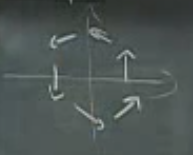
\includegraphics[height=3cm]{21_1.png}

Bir onceki derste bu alanin muhafazakar olmadigina (yani gradyan alani
olamayacagina) karar vermistik, cunku ustteki cember etrafinda bir cizgi
entegrali alinca sonuc sifir degil, pozitif bir deger cikiyordu. Ama biz
yine de, biraz once ogrendigimiz teknigi kullanarak bunu kontrol edelim.

\[ \vec{F} = \underbrace{-y}_{M}\hat{i} + 
\underbrace{x}_{N}\hat{j} 
\]

\[ \frac{\partial M}{\partial y} = -1 \]

\[ \frac{\partial N}{\partial x} = 1 \]

Bu iki sonuc birbirinin aynisi degil. Demek ki alan bir gradyan alani
degil. 

Ornek

\[ \vec{F} = (4x^2 + axy)\hat{i} + (3y^2 + 4x^2)\hat{j} \]

Hangi $a$ degerleri icin bu alan bir gradyan alani olur? 

\[ M_y = ax \]

\[ N_x = 8x \]

$a=8$. Bu arada, ikinci kismi turevleri birbirine esit yapinca, bu esitlik
her noktada dogru olmalidir. Yani cebirsel olarak $ax = 8x$ seklinde bir
esitlik hazirlayip cebirsel numaralarla $x$'i bulmuyoruz, cunku bu cebirsel
cozumde $x=0$ da islerdi, ama bu dogru cevap olmazdi. Biz ikinci kismi
turevlerin ``ayni ifade'' olmasini istiyoruz.

Devam edelim. Alanimiz artik soyle

\[ \vec{F} = (4x^2 + 8xy)\hat{i} + (3y^2 + 4x^2)\hat{j} \]

Peki bu gradyan alaniniyla baglantili potansiyel alani nasil buluruz? 

Bir yontem tahmin etmektir, cogunlukla ise yarar. Ama daha sistematik olan
iki yontem gorecegiz simdi, sinavda bunlardan birini kullanin, cunku tahmin
her zaman ise yaramiyor, hatta bazi durumlarda tahmin yanlis yollara bile
goturebiliyor. 

1. Yontem - cizgi entegralini hesaplayarak 

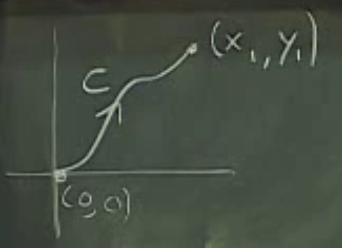
\includegraphics[height=4cm]{21_2.png}

Alanimizda cizgi entegral alalim, benim en favori noktam, orijinden
baslasin, $x_1,y_1$ noktasina giden $C$ uzerinde yapilan isi hesaplasin.
Sonuc soyle olmali

\[ \int_C \vec{F} \cdot d\vec{r} = 
f(x_1,y_1) - f(0,0)
\]

Eger bu dogruysa sunu da yazabilmeliyim (basit bir cebirsel manipulasyon)

\[ f(x_1,y_1) = \int_C \vec{F} \cdot d\vec{r} + f(0,0) \]

ki $f(0,0)$ bir sabittir. Bu sabitin ne oldugunu bilmiyoruz, ama onun ne
olacagini aslinda ``tanimlayabiliriz''. 

Diyelim ki bir potansiyel fonksiyonumuz var. Bu fonksiyona 1 eklemek, ya da
hernangi baska bir sayi eklemek bu potansiyeli degistirmez, cunku
gradyanlar ayni kalacaktir (sabitler kismi turev alinirken yokolacagi
icin). o zaman $f(0,0)$'i bu eklenen sabit olarak gorebiliriz, ya da
entegrasyon sabiti olarak gorebiliriz. Aynen Calculus'ta anti-turev
alindigi zaman oldugu gibi, cebirsel olarak elde edilen formul ``sabit
haricinde'' elde edilen bir sonuctur. 

Fakat ustteki ihtiyaclar baglaminda, bir entegral alinmistir, ama sabit
haricinde formulde geri kalan aradigimiz potansiyel fonksiyonu olarak
gorulebilir. 

O zaman cizgi entegralini hesaplayacagiz. Bu hesapta ustteki resimdekinden
daha basit bir $C$ kullanmak daha iyi olur, mesela soyle (sari cizgi)

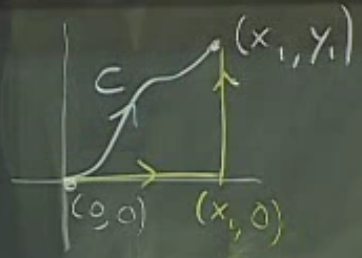
\includegraphics[height=4cm]{21_3.png}

Bu $C$ niye daha basit. Cunku iki parcanin ayri ayri entegralini alirken,
bir parcada $dy$, diger parcada $dx$ sifir olacak, cunku o eksende degisim
olmayacak, boylece cebirsel olarak isimiz daha kolaylasacak. 

Parcalari soyle tanimlayalim

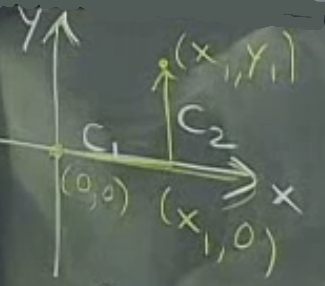
\includegraphics[height=3cm]{21_4.png}

\[ \vec{F} = <4x^2 + 8xy, 3y^2 + 4x^2>\]

Entegal

\[ \int_C \vec{F} \cdot d\vec{r} = 
(4x^2 + 8xy) dx + (3y^2 + 4x^2) dy
\]

Parca $c_1$: $x$, 0'dan $x_1$'e gidiyor, $y=0$, $dy = 0$

\[ \int_{c_1} \vec{F} \cdot d\vec{r} = 
\int_0^{x_1} 4x^2 dx 
\]

Bir suru terim iptal oldu ve bu sayede ustteki ifade bayagi basitlesti. 

Bu arada niye $x,y$ yerine $x_1,y_1$ kullandigim herhalde belli oluyor,
$x,y$ entegrasyon degiskenlerim, $x_1,y_1$ ise sabitler. Neyse, sonuc

\[ = \frac{4}{3} x_1^3\]

Parca $c_2$: $y$, 0'dan $y_1$'e gidiyor, $x=x_1$, $dx = 0$. 

\[ \int_{c_2} \vec{F} \cdot d\vec{r} = 
\int_0^{y_1} (3y^2 + 4x_1^2) dy
\]

\[ = \bigg[ y^3 + 4x_1^2y \bigg]_0^{y_1} \]


\[ = y_1^3 + 4x_1^2 \]

Bu iki sonucu birbirine ekleyince potansiyelin formulu ortaya cikacak.

\[ f(x_1,y_1) = \frac{4}{3} x_1^3 + y_1^3 + 4x_1^2 + c\]

Formuldeki $c$ bir sabit, bastan beri oldugunu farzettigimiz entegrasyon
sabiti bu. 

Bu noktada $x_1,y_1$ yerine $x,y$ da kullanabiliriz artik

\[ f(x,y) = \frac{4}{3} x^3 + y^3 + 4x^2 + c\]

Bu sonucu kontrol edebilirsiniz, eger gradyani alirsaniz, ilk bastaki
vektor alanini elde edersiniz. 

2. Yontem - anti turevleri kullanarak

Oyle bir fonksiyon ariyoruz ki 

\[ 
\left\{ \begin{array}{l}
f_x = 4x^2 + 8xy \\
f_y = 3y^2 + 4x^2
\end{array} \right.
 \]

dogru olmali. 

1. formulu $x$'e gore entegre edelim. 

\[ f = \frac{4}{3}x^3 + 4x^2y + g(y) \ \ \ (*)\]

Burada $g(y)$ entegrasyon sabiti gibi, ama tam degil, cunku $y$ degiskenine
bagli. Ama yine de ilerleme kaydetmis sayiliriz cunku $g(y)$ en azindan
$x$'e bagli degil. 

Simdi ustteki $f$'in $y$'ye gore kismi turevini alirsam ne olur? 

\[ f_y = 4x^2 + g'(y) \]

Bu formulu uc formul ustteki bloktaki $f_y$ ile uydurmak istiyorum
simdi. Bu uydurma bana $g'(y)$'nin ne oldugunu soyleyecek. 

\[ 4x^2 + g'(y) = 3y^2 + 4x^2 \]

ise, o zaman

\[ g' = 3y^2 \]

\[ g(y) = y^3 + c \]

Bu sefer sabit $c$ gercek bir sabit, yani bir sayi, cunku $g$ fonksiyonu
$y$ haricinde baska hicbir seye bagli degil. 

Devam edelim, ustteki formulu alip (*)'a sokarsak

\[ f = \frac{4}{3}x^3 + 4x^2y + y^3 + c\]

Ve daha once 1. yontem sirasinda soyledigimiz gibi, $c$ olmasa da olur,
formulun geri kalani aradigimiz potansiyel alan icin yeterli. 

Bu yontemin avantaji hic entegral tanimi yazmamiza gerek yok. Ama islemleri
dikkatli yapmamiz lazim. 

Bu arada, $g'$'yi uydurduktan sonra eger formul icinde bir $x$ gorursek,
bir seyler yanlis gitmis demektir, belki de aradigimiz alan muhafazakar
degil. 

Notasyon 

Kapali bir egri, yani basi ve sonu birlesen bir egri uzerinden entegral
alininca, bu kapaliligin bariz olmasi icin cogunlukla entegral isareti
degistirilir ve soyle kullanilir 

\[ \oint_{C} \vec{F} \cdot d\vec{r} = 0\]

Yani entegral isaretinin uzerinde bir cember var. Bu notasyon hesaplamada
hicbir sey degistirmiyor, sadece hatirlatici olarak kullaniliyor. 

Ekler

Gradyan alani var ise, her noktada $M_x = M_y$ olmali demistik. Bu ifadeye
tersinden bakarsak o da gecerli olur mu? Yani her noktada $M_x = M_y$ ise
gradyan alani olmali mi? Evet, \underline{ama} eger $\vec{F}$ tum duzlemde
tanimli ise, ya da bir diger deyisle, basitce bagli bolgede (simply
connected region) isek. Basitce bagli bolgelerin tanimi bir dahaki derste. 

Tanim

Rotasyonel operator, Curl'un ne oldugunu gorelim simdi. 

\[ curl(\vec{F}) = N_x - M_y \]

Yani bunlar zaten elimizde olan bilgiler, sadece bu bilgiyi degisik bir
sekilde paketledik, tek bir sayi haline getirdik. 

$M_x = M_y$ sartini $curl(\vec{F}) = 0$ olarak ta ifade edebiliriz. Curl'un
olctugu bir vektor alaninin muhafazakar olmaktaki basarisizligidir. Baska
bir deyisle muhafazakarligin testi $curl(\vec{F})$'in sifir olup olmadigi. 

Bu kavrami zihnimizda canlandirabilmek icin bir hiz alanini
dusunelim. Boyle bir alanda curl rotasyonu olcer. Curl gidisat sirasina ne
kadar bukulme /  kivrilma (twisting) oldugunu olcer, burada Ingilizce satafatli bir
tanim ``vorticity''. 

Diyelim ki bir sabit vektor alanindayim, tum vektorler ayni

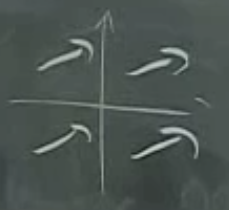
\includegraphics[height=2cm]{21_5.png}

\[ \vec{F} = <a,b> \]

O zaman curl tabii ki sifir, cunku kismi turevleri alinca ikisi de sifir
olacak. Ve resimden de bariz oldugu uzere, bu alanda hic kivrilma bukulme
yok. 

Ya da radyal vektor alanina bakalim

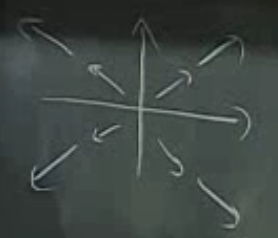
\includegraphics[height=2cm]{21_6.png}

\[ \vec{F}= <x,y> \]

\[ curl \ \vec{F} = \frac{\partial }{\partial x}(y) -
 \frac{\partial }{\partial y}(x) = 0
 \]

ve hakikaten bu alanda da hic rotasyon yok. 

Diger yandan bizim favori alana bakarsak

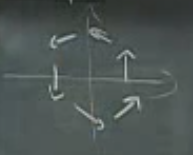
\includegraphics[height=3cm]{21_1.png}

\[ \vec{F} = <-y,x> \]

\[ curl \ \vec{F} = \frac{\partial }{\partial x}(x) -
 \frac{\partial }{\partial y}(-y) = 2
 \]

Bu hareket birim acisal hizda hareket eder, ve curl rotasyon bileseninin
acisal hizinin iki katini hesaplar.

Bir hareketin bilesenlerini dusunursek, mesela bir yerden bir yere tasinma
(translation), yayilma (dilation), rotasyon, vs. Curl bu bilesenlerden
bir noktada rotasyonun ne kadar yuksek oldugunu olcer. 

Cetrefil bir hareket tabii ki her noktada farkli rotasyon sergileyebilir,
bu sebeple zaten curl belli bir noktada olculur, sabit olmasi sart
degildir, her yerde degisebilir. Mesela atmosferik modellemede curl'un
yuksek oldugu bolgeler bir kasirga olabilir. 

Curl'un isareti rotasyonun saat yonunde olup olmadigini belirler. 

Tum bunlarin kuvvet alani baglaminda anlami nedir? Cunku bastan beri kuvvet
alani, orada yapilan isten bahsediyoruz. 

Bir kuvvet alaninin curl'u herhangi bir noktaya koyulabilecek bir test
objesi uzerinde uygulanacak donme kuvvetini (torque) olcer. Hatirlayalim,
donme kuvveti bir kuvvet alaninin rotasyonel dunyadaki karsiligidir. Benzer
sekilde acisal hiz (angular velocity) ve hiz, kutle ve hizlanma egilimi
(moment of inertia) arasindaki parallellik oldugu gibi. 

Kuvvet / kutle bize ivmeyi verir, ki bu hizin turevidir. Donme kuvveti /
hizlanma egilimi bize acisal ivmeyi verir, ve acisal hizin turevidir. 


















\end{document}
